\documentclass[border=3pt]{standalone}
% Shared by the independently buildable vector figures.
\usepackage[T1]{fontenc}
\usepackage{amsmath,amssymb,newpxtext,newpxmath}
\usepackage[semibold]{sourcesans}
\usepackage{pgfplots}
\pgfplotsset{compat=1.18}
\usetikzlibrary{arrows.meta,calc,positioning}
\usepgfplotslibrary{groupplots}
\definecolor{ink}{HTML}{19303A}
\definecolor{sea}{HTML}{00675E}
\definecolor{clay}{HTML}{A24725}
\definecolor{muted}{HTML}{4C636C}
\definecolor{rulegray}{HTML}{CAD4D4}
\definecolor{wash}{HTML}{EAF4F0}
\definecolor{warm}{HTML}{F7EEE5}
\color{ink}
\tikzset{every picture/.style={font=\sffamily\small},
  arrow/.style={-{Stealth[length=2mm]},line width=.8pt,draw=muted}}
\pgfplotsset{companion/.style={axis lines=left,axis line style={draw=muted},
  tick style={draw=muted},ticklabel style={font=\sffamily\footnotesize,text=muted},
  label style={font=\sffamily\small},grid=major,grid style={draw=rulegray!64,line width=.25pt},
  tick align=outside,enlarge x limits=false,scaled ticks=false,
  every axis plot/.append style={line join=round},
  legend style={draw=none,fill=none,font=\sffamily\footnotesize},
  title style={font=\sffamily\bfseries\small,anchor=south west,at={(0,1.03)}}}}

\begin{document}
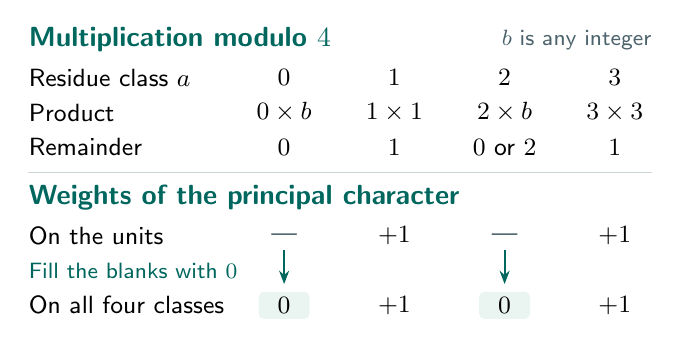
\begin{tikzpicture}[x=1cm,y=1cm,
  row name/.style={anchor=west,inner sep=0pt},
  heading/.style={row name,font=\sffamily\bfseries,text=sea}]
\node[heading] at (0,0) {Multiplication modulo $4$};
\node[anchor=east,inner sep=0pt,text=muted,font=\sffamily\footnotesize]
  at (7.92,0) {$b$ is any integer};
\node[row name] at (0,-.48) {Residue class $a$};
\node[row name] at (0,-.92) {Product};
\node[row name] at (0,-1.36) {Remainder};
\draw[rulegray] (0,-1.68) -- (7.92,-1.68);
\node[heading] at (0,-2.00) {Weights of the principal character};
\node[row name] at (0,-2.49) {On the units};
\node[row name,font=\sffamily\footnotesize,text=sea] at (0,-2.93) {Fill the blanks with $0$};
\node[row name] at (0,-3.37) {On all four classes};

\foreach \x/\residue/\factor/\remainder in {
  3.25/0/b/{$0$},4.65/1/1/{$1$},
  6.05/2/b/{$0$ or $2$},7.45/3/3/{$1$}}{
  \node at (\x,-.48) {$\residue$};
  \node at (\x,-.92) {$\residue\times\factor$};
  \node at (\x,-1.36) {\remainder};
}
\foreach \x in {3.25,6.05}{
  \node[text=muted] at (\x,-2.49) {\textemdash};
  \draw[-{Stealth[length=1.7mm]},draw=sea,line width=.7pt]
    (\x,-2.67) -- (\x,-3.10);
  \node[rounded corners=2pt,fill=wash,minimum width=6.5mm,inner sep=2pt]
    at (\x,-3.37) {$0$};
}
\foreach \x in {4.65,7.45}{
  \node at (\x,-2.49) {$+1$};
  \node at (\x,-3.37) {$+1$};
}
\end{tikzpicture}
\end{document}
